\section{Dense}
Tam bağlı olarak da adlandırılır, çünkü her bir giriş düğümünün her bir çıkış düğümüyle bağlantılı olduğu bir katmandır. Dense katmanının çıkışı, giriş verileri (x) ve ağırlıkları (W) ile bias (b) terimlerinin matris çarpımının sonucu olarak hesaplanır ve ardından bir aktivasyon fonksiyonuna geçirilir.

\begin{figure}[h]
    \centering
    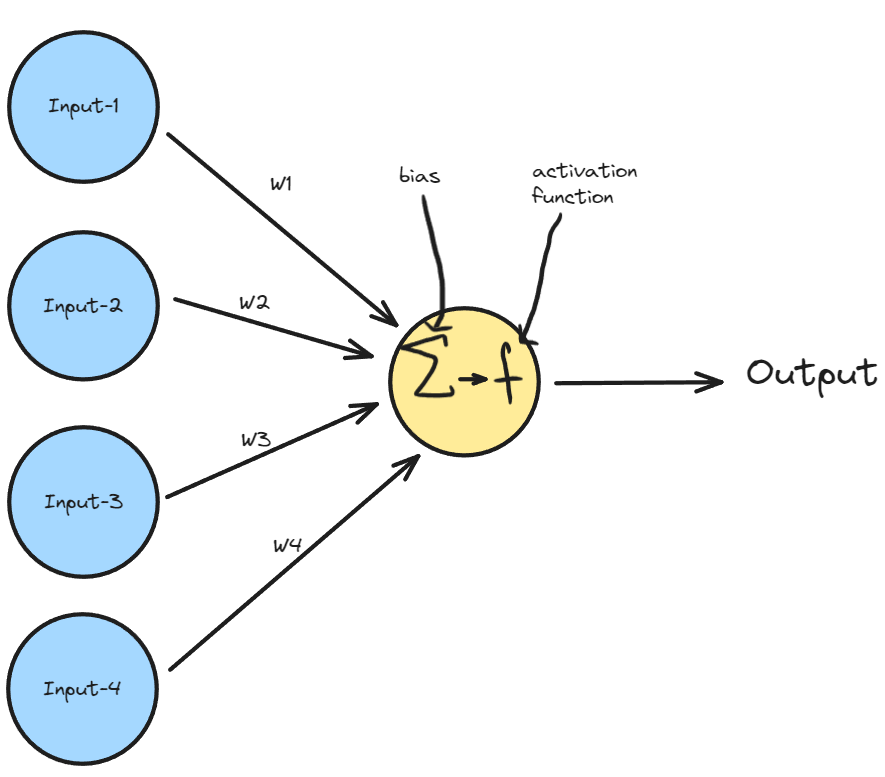
\includegraphics[width=1\textwidth]{images/dense_layer.png}
    \caption{Dense katmanı.}
    \label{fig:enter-label}
\end{figure}

\[\text{AktivasyonFonksiyonu(W * x + b)}\]
x = Giriş \\
b = Bias \\
W = Ağırlık \\

\subsubsection{Çalışma Adımları}
\begin{enumerate}
    \item Önce giriş verileri ile ağırlıklar çarpılır.
    \item Elde edilen sonuca bias eklenir.
    \item Sonuç bir aktivasyon fonksiyonundan geçirilir ve çıkış üretilir.
\end{enumerate}

\subsubsection{Hiperparametreler}
\begin{table}[h]
\centering
{\scriptsize\renewcommand{\arraystretch}{0.4}
{\resizebox*{\linewidth}{0.5\textwidth}{
\begin{tabular}{|p{3cm}|p{6cm}|}
\hline
Parametre & Açıklama \\ \hline
units & Katmandaki gizli nöron sayısıdır yani çıkış boyutunu belirtir. Ağın karmaşıklığını belirler. Daha fazla nöron, öğrenme yeteneğini artırabilir fakat overfitting riskini de artırabilir. \\ \hline
activation & Kullanılacak aktivasyon fonksiyonu. Eğer herhangi bir şey belirtilmezse aktivasyon uygulanmaz. \\ \hline
use\_bias & Bias kullanıp kullanmayacağını belirtir. \\ \hline
kernel\_initializer & Ağırlıkların başlangıç değerlerini belirtir. \\ \hline
bias\_initializer & Bias'ın başlangıç değerini belirtir. \\ \hline
activity\_regularizer & Çıktı üzerindeki düzenleyici. \\ \hline
kernel\_constraint & Ağırlıklar üzerinde uygulanacak sınırlayıcı. \\ \hline
bias\_constraint & Bias üzerinde uygulanacak sınırlayıcı. \\ \hline
bias\_regularizer & Bias üzerindeki düzenleyici. \\ \hline
kernel\_regularized & Kernel üzerindeki düzenleyici. \\ \hline

\end{tabular}
}}}
\end{table}

\newpage